\section{Relacionando expectativa de vida con regresores}

\subsection{Analisis General}
Vamos a querer predecir la expectativa de vida utilizando Cuadrados Mínimos Lineales con distintos regresores. Observamos la tabla de correlación de las variables para tener una idea de cuáles regresores serán más útiles para el modelo, intentando elegir los que mejor se relacionen a la expectativa de vida y a su vez tengan poca correlación entre ellos.


 \begin{figure}[H]
	\centering
	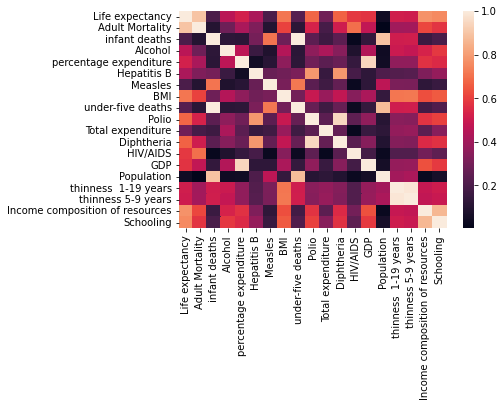
\includegraphics[width=0.7\textwidth]{img/heatmap_corr.png}
	\caption{Heatmap de la matriz de correlación de las variables (en valor absoluto).}
	\label{heatmap}
\end{figure}
        
Viendo la Figura \ref{heatmap} podemos  obtener una primera intuición sobre cuáles variables funcionarán mejor como regresores y cuáles no aportarán mucho al modelo. En principio podemos ver que variables como Adult Mortality e Income composition of resources están muy relacionadas a Life expectancy y serán buenos predictores, mientras que otras como Population, Measles e infant deaths no parecen aportar mucho.
 \begin{figure}[H]
	\centering
	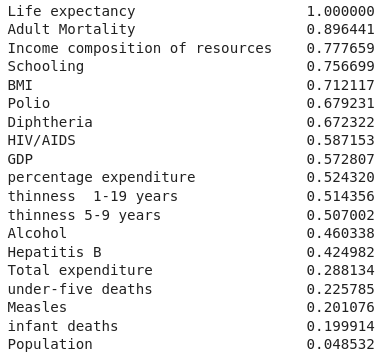
\includegraphics[width=0.45\textwidth]{img/life_exp.png}
	\caption{Correlación entre cada variable y Life Expectancy}
	\label{corr}
\end{figure}

En la Figura \ref{corr} podemos ver cuáles son las variables que más explican la expectativa de vida. Nos interesará elegir algunas de estas variables para la predicción, intentando mejorar las distintas métricas pero a la vez usando la menor cantidad de regresores posibles, buscando disminuir la multicolinealidad. Para eso será necesario tener la menor correlación posible entre las variables utilizadas. Además para la elección de los regresores tendremos en cuenta algunas métricas útiles como el R2 ajustado, el RSE y el VIF para medir la colinealidad. Notamos que usamos los datos normalizados, restando a cada regresor su media y dividiéndolo por su desvío estándar. También agregamos una nueva variable logGDP.


\subsubsection{V1}

Para nuestra primera versión del modelo observamos las variables que están más relacionadas a la expectativa de vida. Comenzamos con un solo regresor y luego vemos cómo mejora el modelo agregando más variables. Para empezar utilizamos Income composition of resources que es una de las variables más relacionada a expectativa de vida. No utilizamos Adult Mortality porque la mortalidad adulta como concepto se relaciona de manera muy directa con la expectativa de vida y nos parece más interesante la relación con Income Composition que tiene en cuenta diversas variables económicas de los países.

Para nuestra primer regresor observamos como dan las métricas con las variables que vimos que están mas correlacionadas a expectativa de vida. Esperamos que Income composition of resources sea de los mejores predictores ya que es el que tiene mayor correlación. Efectivamente el que obtuvo mejores métricas fue el Income composition of resources, con los siguientes valores:

Income composition of resources:

R2: [0.60475395]
R2 ajustado: [0.60257027]
RSE: [5.79131289]



\subsubsection{V2}

En la segunda iteración nos interesa agregar otro regresor que explique mejor el modelo y mejore las métricas, en lo posible incrementando el R2 ajustado y disminuyendo el RSE, y que tenga poco VIF. Observando las variables vemos que la siguientes variables mas relacionadas a Life Expectancy son logGDP y Schooling, pero también sabemos que Income Composition of Resources y Schooling tienen alta correlación por lo que es probable que Schooling no aporte mucho al modelo. De hecho, el VIF entre estas dos variables es de 3.9476, bastante alto. Tiene sentido, considerando que los países con mayor bienestar económico tendrán mejores posibilidades para brindar acceso a la educación. Efectivamente vemos que al agregar Schooling obtenemos un R2 ajustado de 0.629. Por otra parte logGDP devuelve un R2 ajustado de 0.65 y un VIF de 2.954 que también es bastante alto.

Con las variables BMI, Polio, y Diphtheria obtenemos valores de VIF (calculados por separado, junto al ICR) de [1.66, 1.49 y 1.437 son los de Difteria, Polio, Hep B; respectivamente]; y de R2 ajustado 0.682, 0.681 y 0.686. Estos valores no están tan mal pero tampoco mejoran mucho el R2 ajustado.

A diferencia de con estas variables, el IRC tiene poca correlación con el indicador HIV/AIDS: el VIF da 1.098. A su vez, el modelo incorporando a esta variable mejora su R2 ajustado hasta el valor de 0.7399. Por un lado, vemos que incorporar este feature, aunque tenga menos correlación con la expectativa de vida que otras (como Schooling, BMI, etc.), aumenta en mayor medida el R2 ajustado. Esto se explica justamente por la baja colinealidad entre ella e IRC. Queda como una pregunta abierta cuál es específicamente la información que agrega esta variable al modelo. No creemos que la cantidad de muertos por VIH/SIDA sea tan grande como para afectar en sí misma a la expectativa de vida de forma significativa. Entonces, debe ser expresión de un fenómeno que sí la afecte notoriamente. Por lo visto anteriormente, parece no estar tan relacionado con el bienestar económico. Quedará pendiente para futuras investigaciones.   

% Algo interesante sucede agregando la variable HIV/AIDS, obteniendo un R2 ajustado de 0.739, a pesar de que HIV/AIDS tiene menos correlación con Life Expectancy que las variables ya mencionadas. Esto se puede explicar debido a que la correlación entre Income Composition y HIV/AIDS es menor que con las otras variables, por lo que el uso de HIV/AIDS aporta información útil al modelo con menor colinealidad. 

Predictor: ['Income composition of resources', 'HIV/AIDS']

Resultados de las métricas:

R2: 0.74276834

R2 ajustado: 0.73991021

RSE: 4.67202835

VIF: 1.0983151726267792

\subsubsection{Vn}

En iteraciones subsiguientes vamos a querer seguir agregando variables que estén poco relacionadas a los regresores ya utilizados y que a su vez se relacionen de alguna manera con la expectativa de vida. Por ejemplo, agregando Polio o Diphtheria el R2 ajustado aumenta al 0.802, 0.807. Observamos que agregar ambas variables (Polio y Diphtheria) no será muy útil ya que tienen alta correlación, y efectivamente vemos que obtenemos un R2 ajustado de 0.807 que es equivalente a agregar sólo Diphtheria. La siguiente variable que parece mejorar las métricas es BMI obteniendo un R2 ajustado de 0.834 y un VIF razonable de 1.804. Luego de esto no mejora mucho el R2, a los sumo agregando percentage expenditure que obtenemos un R2 ajustado de 0.8487350 y además obtenemos un menor VIF de 1.491986.
A partir de esta ultima inclusión no encontramos beneficio en agregar más variables ya que en todos los casos las métricas empeoraron o se mantuvieron iguales, probablemente porque están relacionadas a los regresores ya utilizados y no tengan mucho para aportar al modelo.

Un predictor final podría ser:
['Income composition of resources', 'HIV/AIDS', 'Diphtheria', 'BMI', 'percentage expenditure']


Resultados de las métricas:

R2: [0.8528907]

R2 ajustado: [0.84873507]

RSE: [3.53316018]

VIF: 1.491986365304516

\subsection{Análisis Por Categorias: Developing}

Observamos que podemos partir nuestro dataset en dos grandes grupos: países desarrollados y países en vías de desarrollo, y que esta división probablemente sea útil para el análisis de regresores. Partimos el dataset en dos y observamos sus características, comenzando con los países en vías de desarrollo.

 \begin{figure}[H]
	\centering
	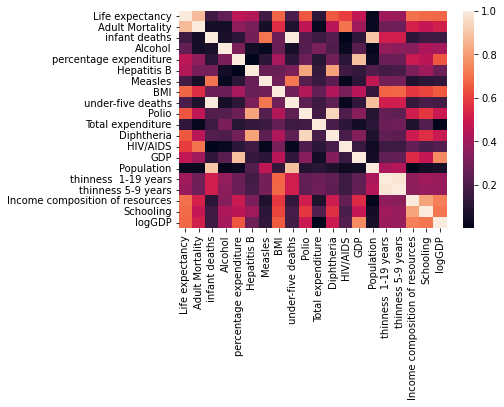
\includegraphics[width=0.7\textwidth]{img/heatmap_corr_developing.png}
	\caption{Heatmap de la matriz de correlación de las variables en países en vías de desarrollo (en valor absoluto).}
	\label{heatmap_developing}
\end{figure}

 \begin{figure}[H]
	\centering
	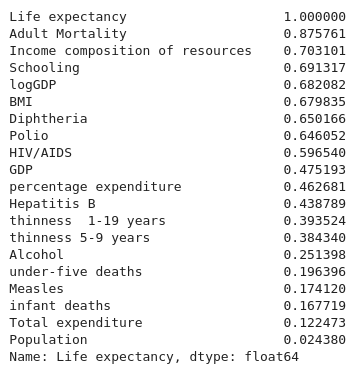
\includegraphics[width=0.5\textwidth]{img/tabla_developing.png}
	\caption{Tabla de correlaciones en países en vías de desarrollo.}
	\label{tabla_developing}
\end{figure}

A simple vista podemos ver que en términos generales el modelo es bastante parecido al utilizado en el caso general, esto puede deberse a que los países en vías de desarrollo son mayoría y por eso se parece mucho al caso global. Esperamos ver resultados mas particulares en el análisis de países desarrollados.

\subsubsection{V1}

Como primer regresor eligiremos al que tenga mejores métricas y explique mejor a la expectativa de vida. Comparamos las métricas R2/R2 ajustado y RSE entre las variables mas relacionadas con expectativa de vida y obtenemos de vuelta a Income composition of resources como el mejor regresor.

Income composition of resources:

R2: [0.49435129]
R2 ajustado: [0.49095768]
RSE: [6.15956382]

Observamos que comparado con el caso general, ahora ICR no explica tan bien al modelo (R2 de [0.60475395] a [0.49435129] y RSE de 5.7 a 6.15) lo cual tiene sentido ya que en la tabla de correlaciones vemos que la correlacion también es menor (de 0.77 a 0.70.)

\subsubsection{V2}

En la segunda iteración observamos que variable podemos agregar que mejore las métricas y ayude a explicar el modelo. Analizando las variables mas importantes (las mas relacionadas a expectativa de vida) sucede algo parecido al caso de análisis general donde la variable que mejora mas las métricas es HIV/AIDS con un R2 ajustado de 0.676, un RSE de 4.89 y un VIF de 1.06. Esto es interesante ya que en este caso HIV/AIDS es la variable numero 8 en término de relación con expectativa de vida, pero al estar muy poco relacionada con Income composition of resources es la que mejor explica el modelo. Por ejemplo, ICR y Schooling (la segunda mas relacionada a life exp) tiene R2 ajustado de 0.528, RSE de 5.9 y VID de 3.024, lo cual era esperable porque ICR y Schooling estan altamente relacionadas, por lo que un segundo predictor podría teniendo en cuenta ICR y HIV/AIDS

% Algo interesante sucede agregando la variable HIV/AIDS, obteniendo un R2 ajustado de 0.739, a pesar de que HIV/AIDS tiene menos correlación con Life Expectancy que las variables ya mencionadas. Esto se puede explicar debido a que la correlación entre Income Composition y HIV/AIDS es menor que con las otras variables, por lo que el uso de HIV/AIDS aporta información útil al modelo con menor colinealidad. 

Predictor: ['Income composition of resources', 'HIV/AIDS']

Resultados de las métricas:

R2: [0.53510995]

R2 ajustado: [0.52882765]

RSE: [5.9060978]

VIF: 3.024119900228316

\subsubsection{Vn}
En las siguientes iteraciones hacemos un proceso similar para ir agregando regresores, viendo en cada caso cual ayuda a explicar mejor el modelo buscando la menor correlacion entre los regresores y evitando la multicolinealidad (manteniendo un VIF bajo, al menos \< 5). En la búsqueda del tercer regresor encontramos los mejores resultados agregando Diphtheria y en el 4to agregando BMI, obteniendo un R2 ajustado de 0.81, un RSE de 3.723 y un VIF de 1.6265. Finalmente analizando un quinto regresor vemos que quizás se podría agregar percentage expenditure con un R2 ajustado de 0.8167, un RSE de 3.64 y un VIF de 1.373, pero comparando con la 4ta iteración vemos que no mejoran mucho las métricas por lo que un predictor final podría utilizar ICR, HIV/AIDS, Diphtheria, y BMI.

Predictor:
['Income composition of resources', 'HIV/AIDS', 'Diphtheria', 'BMI']

Metricas:

R2: [0.81519655]

R2 ajustado: [0.81013344]

RSE: [3.72375024]

VIF: 1.6265061009609258

\subsection{Análisis por Categorías: Developed}

Tomamos el conjunto de países desarrollados y observamos sus características. 

 \begin{figure}[H]
	\centering
	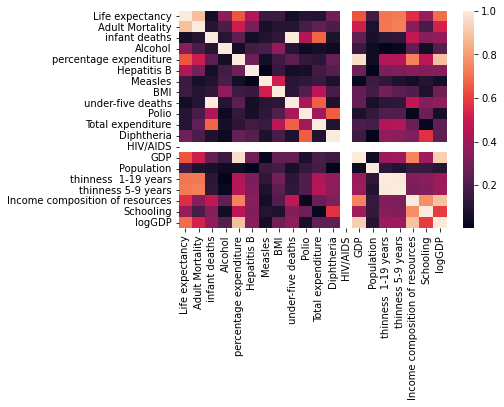
\includegraphics[width=0.7\textwidth]{img/heatmap_corr_developed.png}
	\caption{Heatmap de la matriz de correlación de las variables en países dessarrollados (en valor absoluto).}
	\label{heatmap_developed}
\end{figure}

 \begin{figure}[H]
	\centering
	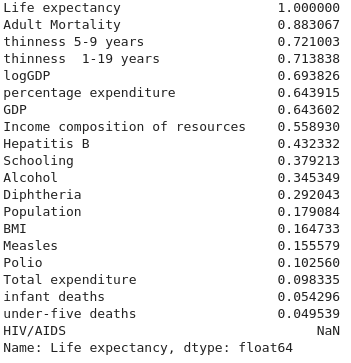
\includegraphics[width=0.4\textwidth]{img/tabla_developed.png}
	\caption{Tabla de correlaciones en países desarrollados.}
	\label{tabla_developed}
\end{figure}


A simple vista vemos que este modelo difiere bastante del análisis general y los países en vías de desarrollo. En primer lugar vemos un comportamiento extraño con la variable HIV/AIDS. Observando los datos vemos que todos los países desarrollados tienen el mismo valor de HIV/AIDS, y al aplicar la normalización de los datos se divide por el desvió estándar (que da 0) y obtenemos NaNs, por lo que desecharemos esta variable y no la tendremos en cuenta.

Podemos ver que hay algunas variables que toman un peso mucho mas importante en el caso de los países desarrollados: thinness 5-9 years y thinness 1-19 years. Sabemos que ambas están altamente correlacionadas por lo que tendremos en cuenta solo una. Nos pareció extraño ya que uno pensaría que en los países desarrollados no hay muchos casos de desnutrición, quizás pueda darse por algún problema regional de desnutrición. Vemos en los datos que los países con peores valores de thinness se encuentran en el este de Europa, países como Rumania, Latvia, Lituania y Bulgaria, esto puede deberse a una cuestión geográfica y también puede estar relacionado a problemas de pobreza y calidad de vida que no ocurren en países del oeste de Europa y se ven reflejados en el índice de desnutrición. 

\subsubsection{V1}

Como primer regresor elegimos thinness 5-9 years que es el que mejor explica la expectativa de vida. Observamos que en el futuro probablemente no agreguemos thinness 1-19 years ya que ambas están altamente correlacionadas. El resto de las variables (logGDP, percentage expenditure, GDP..) no dieron tan buenas métricas por lo que nos quedamos con thinness 5-9 years.

Predictor: ['thinness 5-9']

Metricas: 

R2: [0.51984568]

R2 ajustado: [0.50384054]

RSE: [2.27024552]

\subsubsection{V2}

Observamos las métricas tomando thinness 5-9 years y otras variables para ver cuales aportan mas información al modelo. El regresor con el que obtuvimos las mejores métricas fue logGDP obteniendo los siguientes resultados:

Predictor: ['thinness 5-9' y 'logGDP']

Metricas:

R2: [0.71880595]

R2 ajustado: [0.69941325]

RSE: [1.73734262]

VIF: 1.1833091879040005

\subsubsection{Vn}

En siguientes iteraciones encontramos como el mejor tercer regresor a la variable 'Alcohol' obteniendo valores de R2 ajustado = 0.74865007, RSE = 1.5610613 y 
VIF = 1.0573780269799327 y como cuarto regresor a la variable 'Measles' obteniendo valores de R2 ajustado = 0.75875508, RSE = 1.50180148 y VIF: 1.0506871. En búsqueda de un quinto regresor no encontramos ninguno que mejore las métricas, por lo que nos quedamos con los 4 regresores que tenemos. 

Predictor: ['thinness 5-9 years', 'logGDP', 'Alcohol', 'Measles']

Metricas:

R2: [0.78988346]

R2 ajustado: [0.75875508]

RSE: [1.50180148]

VIF: 1.0506871618402263
